% WatITis Talk 2012 - Colin Bell <colin.bell@uwaterloo.ca>

\documentclass{beamer}
\usepackage{hyperref}
\usepackage{graphicx}
% BEGIN - Beamer settings
\definecolor{watitisred}{RGB}{183,26,55}
\usetheme{Warsaw}
\usecolortheme[RGB={255,218,0}]{structure}
\setbeamercolor{titlelike}{fg=black}
\setbeamercolor{section in toc}{fg=watitisred}
\setbeamercolor{description item}{fg=watitisred}
\setbeamercolor{subsection in head}{fg=watitisred}
\setbeamercolor{local structure}{fg=watitisred}
% END - Beamer settings
\begin{document}
\title{Why API? (and other Architectural Anecdotes)}
\author{Colin Bell\\Director, Enterprise Architecture} 
\institute{Information Systems and Technology (IST), University of Waterloo}
\date{December 3, 2012} 

\frame{\titlepage} 

\frame{\frametitle{Table of contents}\tableofcontents}

%\frame{\frametitle{Licensing}
%In a number of locations I have pulled quotes and images directly from \url{http://wikipedia.org}.  I have attributed direct quotes to their sources throughout the presentation.  
%\\
%To feel confident that I have met my obligations to the awesome folks at wikipedia.org, this presentation is licensed under:\\
%\url{http://creativecommons.org/licenses/by-sa/3.0/}
%}

\section{Why}

\section{"The Cloud"}
\frame{\frametitle{Definition: Cloud Computing}
\begin{quotation}
\emph{\bf{Cloud computing}} is the use of computing resources (hardware and software) that are delivered as a service over a network (typically the Internet). The name comes from the use of a cloud-shaped symbol as an abstraction for the complex infrastructure it contains in system diagrams. Cloud computing entrusts remote services with a user's data, software and computation.\vspace{0.5cm}\\
\end{quotation}
\tiny{Source: \url{http://en.wikipedia.org/wiki/Cloud\_computing}}
}
\frame{\frametitle{Image: Cloud Computing}
\hfill\tiny{Source: \url{http://upload.wikimedia.org/wikipedia/commons/b/b5/Cloud\_computing.svg}}
\begin{center}
%\vspace{-0.3cm}\includegraphics[width=3.25in]{cloudimage}
\end{center}
}

\subsection{Types of Cloud Services}
\frame{\frametitle{Types of Cloud Services}
\begin{itemize}
\item Software as a Service \emph{(SaaS)}
\item Platform as a Service \emph{(PaaS)} 
\item Infrastructure as a Service \emph{(IaaS)}
\end{itemize}
}

\frame{\frametitle{SaaS - Software (Application) as a Service}
\begin{itemize}
\item Software (Application) as a Service \emph{(SaaS)}:
\begin {itemize}
\item providers install and operate application software,
\item very little flexibility, you get what is provided, and;
\item users do not worry about the underlying platform or infrastructure.
\end {itemize}
%%\pause
\item Examples:
\begin{itemize}
\item GMail / Google Apps
\item Hotmail / Microsoft Office 365
\item Salesforce
\end{itemize}
\end{itemize}
}

\frame{\frametitle{PaaS - Platform as a Service}
\begin{itemize}
\item Platform as a Service \emph{(PaaS)}:
\begin {itemize}
\item provides users with an infrastructure pre-configured with a suite of tools,
\item often users are locked into a particular development suite, database, and Web server, and;
\item users can build and run software in a controlled environment.
\end {itemize}
%%\pause
\item Examples:
\begin{itemize}
\item Google App Engine
\item Engine Yard
\item Windows Azure Compute
\end{itemize}
\end{itemize}
}

\frame{\frametitle{IaaS - Platform as a Service}
\begin{itemize}
\item Infrastructure as a Service \emph{(IaaS)}:
\begin {itemize}
\item low-level access to basic computing components,
\item can choose own OS, software stack, and configuration settings, and;
\item clients are given their own virtual networks and data centre.
\end {itemize}
%%\pause
\item Examples:
\begin{itemize}
\item Amazon AWS
\item Rackspace Cloud
\item Joyent
\end{itemize}
\end{itemize}
}

\frame{\frametitle{Economies of Scale Benefits}
\begin{center}
\Huge{SaaS \textgreater PaaS \textgreater IaaS}
\\Why?
\end{center}
%\pause
Less Complexity $+$ Fewer Features
\\ $\implies$ Increased Specialization (decreasing per-unit cost)
\\ $\implies$ Increased benefits from Economies of Scale
}

\subsection{Deployment of Clouds}
\frame{\frametitle{Deployment of Clouds}
\begin{description}
\item[Public Cloud]
Infrastructure that is owned by a corporation who sells their services to the general public.
%%\pause
\item[Community Cloud]
Infrastructure that is shared amongst like-entities.  Municipalities, Governments, non-Profit Organizations, and Non-Governmental Organizations often share these services.
%%\pause
\item[Private Cloud]
Infrastructure that is operated solely for a single entity.
%%\pause
\item[Hybrid Cloud]
A composition of two or more clouds that are separate at the lowest Infrastructure levels while allowing interconnection at higher levels.
\end{description}
}

\subsection{Why Cloud?}
\frame{\frametitle{Value Generation (Impact++) vs. Cost}
\begin{itemize}
\item By increasing the number of customers and improving specialization, the cost of production (of services) can be driven down.
\begin{itemize}
%\pause
\item Economies of scale is kicking in.
\end{itemize}
%\pause
\item When someone else can provide service for less, do we consider the Opportunity Cost?
\begin{itemize}
\item Is maintaining the status quo a good idea?
\end{itemize}
%\pause
\item What 'higher value' things could we be doing to make the organization more productive?
\end{itemize}
}

\frame{\frametitle{1994: Wentworth Research Program}
\begin{center}
%\includegraphics[width=2.6in]{time-to-reshape-it}
\end{center}
\vspace{-0.5cm}\tiny{Source: George Cox, Time to Reshape the IS Department? Wentworth Research Program (now part of Gartner EXP, Stamford, CT), June 1994.}
}

\section{What is a Service?}
\subsection{Definitions}
\frame{\frametitle{What is a Service?}
\begin{description}
\item[Basic Definition]
Inputs + Functionality = Output
%%\pause
\item[Formal Definition]
See: Journal of Software, July 2006 \textgreater Aliaksei Yanchuk, Alexander Ivanyukovich, Maurizio Marchese \\ "Towards a Mathematical Foundation for Service-Oriented Applications Design"
\end{description}
}

\subsection{Practical Definition}
\frame{\frametitle{What is a Service?}
\begin{itemize}
\item Practical Definition ... \vspace{1cm}
\begin{itemize}
\item Inputs = (effort, data, contract, connection)
\item Functionality (unknown to user)
\item Output = (results)
\end{itemize} 
\end{itemize}
}

\subsection{Graphical Representation}
\frame{\frametitle{What is a Service?}
\begin{center}
%\vspace{-0.2cm}\includegraphics[width=3in]{Chorded-Circle}
\end{center}
}

\section{Building the Services Oriented Enterprise (SOE)}
\frame{\frametitle{What is a Services Oriented Enterprise?}
Based on OASIS SOA Reference Model 1.0:
\begin{quotation}
A Services Oriented Enterprise (SOE) is an organization whose business and IT are converged based on the enterprise business service model to gain business goals in the most efficient way in the given market.
\end{quotation}
\emph{\tiny{https://www.oasis-open.org/committees/soa-rm/}}
}

\subsection{Service Management w/ ITIL}
\frame{\frametitle{Information Technology Infrastructure Library (ITIL)}
\begin{description}
\item[Service Strategy]
provides guidance on clarification and prioritization of service-provider investments in services.
\item[Service Design]
provides good-practice guidance on the design of IT services, processes, and other aspects of the service management effort.
\item[Service Transition]
relates to the delivery of services required by a business into live/operational use, and often encompasses the "project" side of IT rather than.
\end{description}
Quotes From: \url{http://en.wikipedia.org/wiki/Information\_Technology\_Infrastructure\_Library}
}

\frame{\frametitle{Information Technology Infrastructure Library (ITIL)}
\begin{description}
\item[Service Operation]
aims to provide leading practice for achieving the delivery of agreed levels of services both to end-users and the customers (where "customers" refer to those individuals who pay for the service and negotiate the Service Level Agreements (SLAs).
\item[Continual Service Improvement]
aims to align and realign IT services to changing business needs by identifying and implementing improvements to the IT services that support the business processes.
\end{description}
Quotes From: \url{http://en.wikipedia.org/wiki/Information\_Technology\_Infrastructure\_Library}
}

\subsection{Enterprise Architecture (EA)}
\frame{\frametitle{Enterprise Architecture (EA)}
\begin{quotation}
\emph{Gartner:\\ \bf{Enterprise architecture (EA)}} is a discipline for proactively and holistically leading enterprise responses to disruptive forces by identifying and analyzing the execution of change toward desired business vision and outcomes. EA delivers value by presenting business and IT leaders with signature-ready recommendations for adjusting policies and projects to achieve target business outcomes that capitalize on relevant business disruptions. EA is used to steer decision making toward the evolution of the future state architecture.\vspace{0.5cm}\\
\end{quotation}
Source: \url{http://www.gartner.com/it-glossary/enterprise-architecture-ea/}
}

\frame{\frametitle{Enterprise Architecture (EA)}
\begin{quotation}
\emph{Human readable:\\ \bf{Enterprise architecture (EA)}}  is a discipline for taking a structured approach to studying, documenting, designing, planning, and facilitating change within an organization. The goal of EA is to allow an enterprise to better identify high-value opportunities and help it effectively capitalize on them.
\end{quotation}
}

\subsubsection{Zachman Framework for Enterprise Architecture}
\frame{\frametitle{Zachman Framework for Enterprise Architecture}
\begin{columns}
\begin{column}{0.5\textwidth}
\begin{flushleft}
Zachman Columns:
\begin{description}
\item["What"]
Things + Data
\item["How"]
Processes
\item["Where"]
Network
\item["Who"]
People
\item["When"]
Events + Times
\item["Why"]
Strategies + Motivations
\end{description}
\end{flushleft}
\end{column}
\begin{column}{0.5\textwidth}
\begin{flushleft}
Zachman Rows:
\begin{description}
\item["Contextual"]
Planner / Enterprise View
\item["Conceptual"]
Owner / Business View
\item["Logical"]
Designer / Architect View
\item["Physical"]
Builder / Engineer View
\item["Detailed"]
Sub-contractor / Technician View
\item["Functional"]
Operator View
\end{description}
\end{flushleft}
\end{column}
\end{columns}
}

\frame{\frametitle{Zachman Framework for Enterprise Architecture}
\begin{center}
%\vspace{-0.7cm}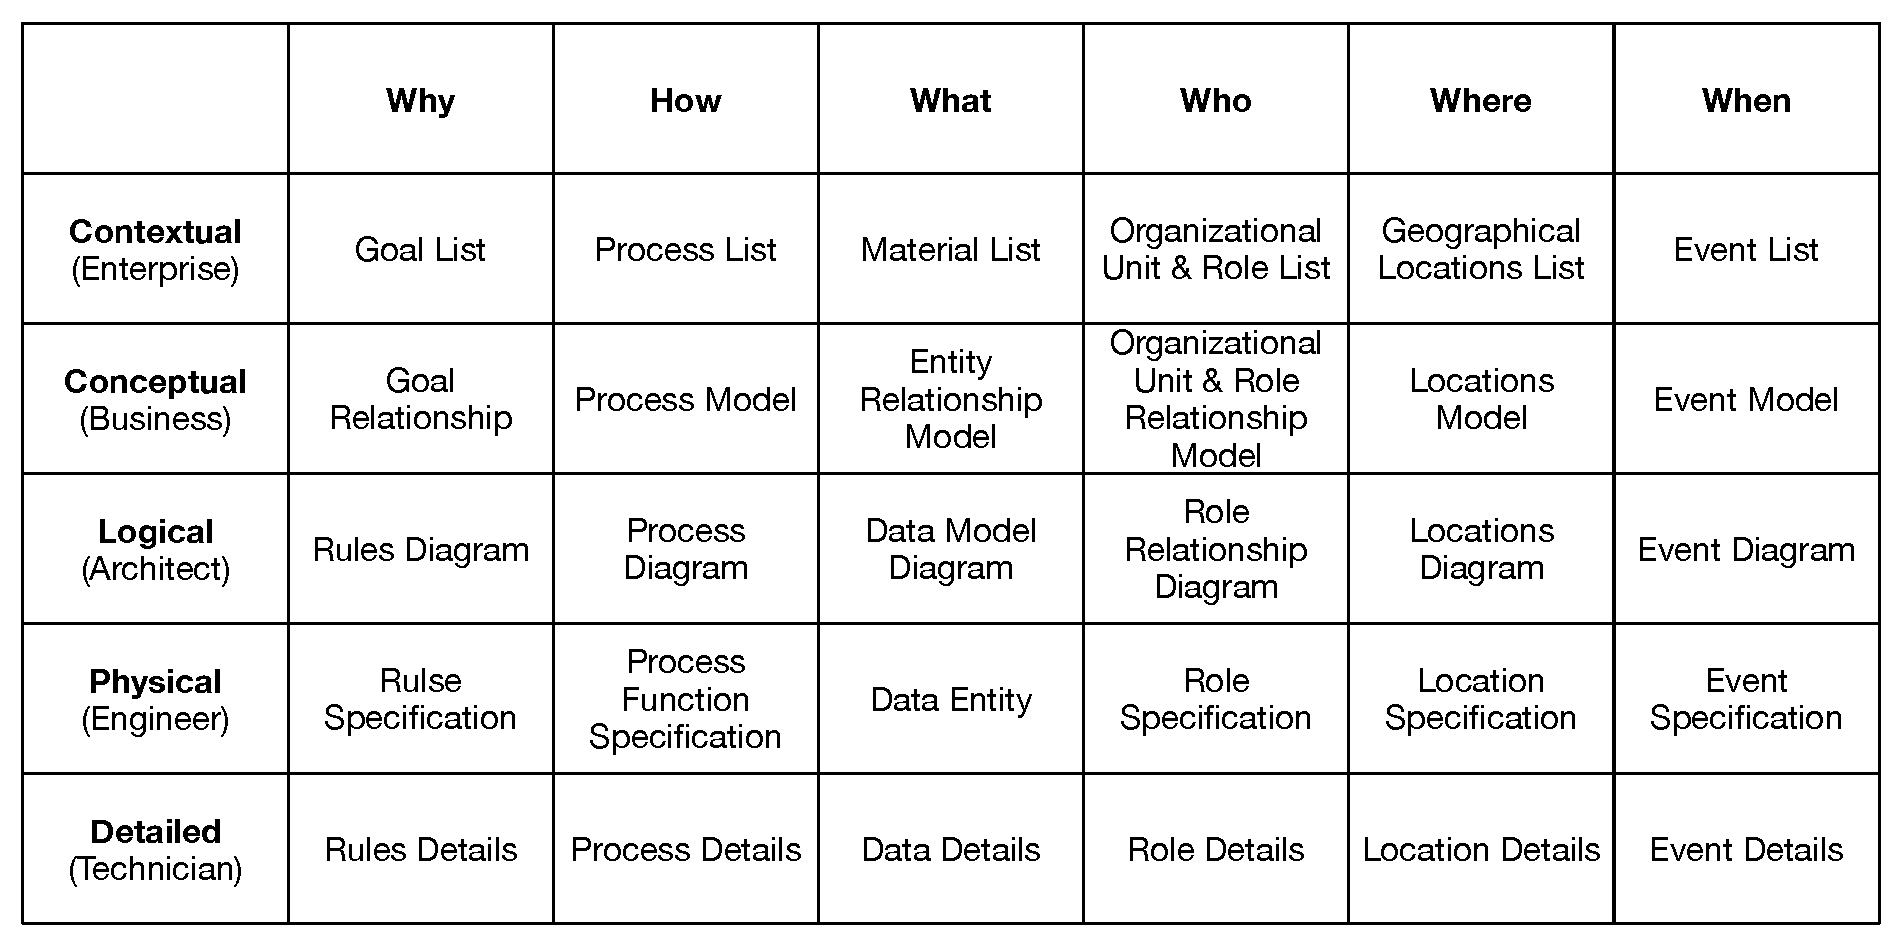
\includegraphics[width=4.5in]{EAWG-Zachman_Matrix}
\end{center}
}

\subsection{Service-Oriented Architectures (SOA)}
\frame{\frametitle{Service-Oriented Architectures (SOA)}
\begin{quotation}
 In software engineering, a service-oriented architecture (SOA) is a set of principles and methodologies for designing and developing software in the form of interoperable services. These services are well-defined business functionalities that are built as software components (discrete pieces of code and/or data structures) that can be reused for different purposes. SOA design principles are used during the phases of systems development and integration."
\end{quotation}
\emph{\tiny{Source: http://en.wikipedia.org/wiki/Service-oriented\_architecture}}
}

\frame{\frametitle{SOA Principles: Quick + Dirty}
\begin{itemize}
\item loosely couple at all costs
\item never require a particular operating system or technology
\item keep services unassociated until runtime
\item do not allow any embedded links between services
\item only communicate over documented channels
\item only communicate through documented interfaces
\item to build on top of other services (compose) at quality and to spec, SLA underpinning contracts (UCs) are required
\end{itemize}
}

\frame{\frametitle{SOA Principles: Thomas Erl View}
\emph{\tiny{From: http://www.soaposters.com/}}
\begin{description}
\item[Standardized Service Contract]
Services within the same service inventory are in compliance with the same contract design standards.
\item[Service Loose Coupling]
Service contracts impose low consumer coupling requirements and are themselves decoupled from their surrounding environment.
\item[Service Abstraction]
Service contracts only contain essential information and information about services is limited to what is published in service contracts.
\end{description}
}

\frame{\frametitle{SOA Principles: Thomas Erl View}
\emph{\tiny{From: http://www.soaposters.com/}}
\begin{description}
\item[Service Reusability]
Services contain and express agnostic logic and can be positioned as reusable enterprise resources.
%%\pause
\item[Service Autonomy]
Services exercise a high level of control over their underlying runtime execution environment.
%%\pause
\item[Service Statelessness]
Services minimize resource consumption by deferring the management of state information when necessary.
\end{description}
}

\frame{\frametitle{SOA Principles: Thomas Erl View}
\emph{\tiny{From: http://www.soaposters.com/}}
\begin{description}
\item[Service Discoverability]
Services are supplemented with communicative meta data by which they can be effectively discovered and interpreted.
%%\pause
\item[Service Composability]
Services are effective composition participants, regardless of the size and complexity of the composition.
\end{description}
}

\frame{\frametitle{Why SOA? Ask Stevey!}
Case: Amazon vs. Google\\
\emph{Steve Yegge's "Stevey's Google Platforms Rant"}\\
\begin{itemize}
\item Engineer at Google released a rant on Google+ around Oct 2011.
%%\pause
\item A user error with Google+ led to a Google employee posting a rant against Google.
%\pause
\item He had worked at Amazon before Google and ranted about where Google was failing.
\end{itemize}
}

\frame{\frametitle{Why SOA? Ask Stevey!}
In 2002, Jeff Bezos (founder + CEO of Amazon) issued a mandate.
\begin{enumerate}
\item All teams will henceforth expose their data and functionality through service interfaces.
%%\pause
\item Teams must communicate with each other through these interfaces
%%\pause
\item There will be no other form of interprocess communication allowed: no direct linking, no direct reads of another team's data store, no shared-memory model, no back-doors whatsoever. The only communication allowed is via service interface calls over the network.
\end{enumerate}
}
\frame{\frametitle{Why SOA? Ask Stevey!}
\begin{enumerate}
\item  It doesn't matter what technology they use. HTTP, Corba, Pubsub, custom protocols -- doesn't matter. Bezos doesn't care.
%%\pause
\item All service interfaces, without exception, must be designed from the ground up to be externalizable. That is to say, the team must plan and design to be able to expose the interface to developers in the outside world. No exceptions. 
\end{enumerate}
}
\frame{\frametitle{Why SOA? Ask Stevey!}
Lessons from a massive undertaking of building SOA at Amazon:
\begin{itemize}
%\pause
\item pager escalation can get hard.  need metrics and reporting
%\pause
\item every single one of your peer teams becomes a potential denial of service
%\pause
\item monitoring and QA are the same thing in SOAs
%\pause
\item a universal service registration mechanism is a powerful thing to have
%\pause
\item follow-on benefits are compelling
\end{itemize}
}
\frame{\frametitle{Why SOA? Ask Stevey!}
\begin{itemize}
\item Steve then explains... as hard as SOA was, it was the Right Thing to do.
%%\pause
\item He goes on to stress that Amazon's abilities as a provider of Infrastructure and a Platform far outstrip Google because of one ultimate thing:
%%\pause
\item \emph{\bf{Accessibility!}} %\pause NOT WCAG Accessibility... %\pause he means fundamental access to information and functionality.
%%\pause
\item If someone should be able to access something and cannot get it through a Service, it represents a HUGE roadblock to the Organization's success.
\end{itemize}
}
\frame{\frametitle{Why SOA? Ask Stevey!}
Moral of the story:\\
There is evidence that an organization is able to thrive in their market after adopting an SOA mandate  They were able to develop marketable value-add functionality following their adoption of SOA. They accomplished this by imposing a requirement that everyone always use 'Services.' Amazon used a series of Lego blocks to combine functionality in a wide variety of ways.
}

\frame{\frametitle{Governance}
\emph{\tiny{From: "IT Savvy: What Top Executives Must Know to Go from Pain to Gain" by Peter Weill and Jeanne W. Ross}}
\small{
\begin{itemize}
\item We need to clarify Waterloo's primary operating model.
\begin{description}
\item[Diversification] 
Low standardization, low integration-- involves platform of shared services that supports autonomous business activities.
\item[Coordination] 
Low standardization, high integration-- involves building a platform of shared data to support integrated management decisions or a single face to the customer.
\item[Replication]
High standardization, low integration-- involves building a platform of standard technologies and business processes to define a common brand.
\item[Unification]
High standardization, high integration-- involves building a platform of standardized technologies, business processes, and shared data to support global end-to-end customer requirements.
\end{description}
\end{itemize}
}
}

\frame{\frametitle{Service Oriented Maturity Model}
\begin{center}
%\vspace{-0.2cm}\includegraphics[width=3in]{soa_maturity_pyramid}
\end{center}
\emph{\tiny{http://www.enterprise-architecture.info/EA\_Services-Oriented-Enterprise.htm}}
}

\frame{\frametitle{Looks crazy, but it's just a series of blocks!}
\begin{center}
%\vspace{-0.2cm}\includegraphics[width=3in]{lego-image}
\end{center}
\emph{\tiny{Image: http://collider.com}}
}

\frame{\frametitle{Injury Time / Q+A}
\begin{itemize}
\item Choreography of Services - the more mature we get, the better we dance.
\item Design
\begin{itemize}
\item Design Top-Down - start from strategy / planning, work down to implementation.
\item Design Bottom-Up - start from an existing implementation, decompose, and re-wrap it.
\end{itemize}
\item Service have Layers - Enterprise Service vs. Domain Service vs. Application Service
\end{itemize}
}

\end{document}
